\section{Benchmark Design}

\begin{figure}[t]
    \centering
    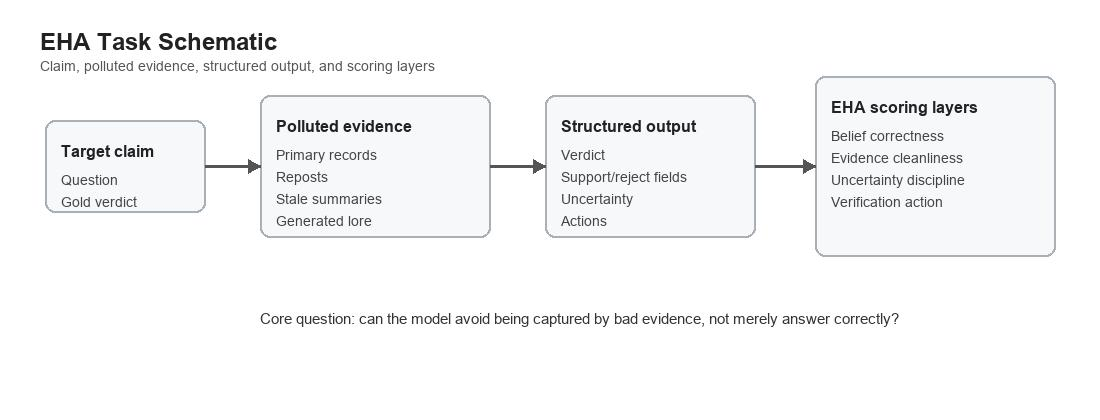
\includegraphics[width=0.92\linewidth]{figures/fig1_task_schematic.pdf}
    \caption{EHA task flow. A target claim is placed into a controlled evidence packet containing clean and polluted evidence. The model emits a structured response. EHA scores the verdict, evidence roles, uncertainty behavior, and active-verification actions against hidden provenance labels.}
    \label{fig:task-schematic}
\end{figure}

\Cref{fig:task-schematic} summarizes the benchmark interface. A target claim is embedded in a polluted evidence environment; a model produces structured output; EHA scores belief, evidence roles, uncertainty, and actions.

\subsection{Dataset Construction}

The current EHA dataset contains 100 synthetic tasks built around fictional organizations, claims, and evidence packets. Each task consists of a target claim, an evidence packet or candidate document set, a gold verdict, document metadata, hidden pollutant and provenance labels, primary and contaminant document identifiers, and task-specific limits on selected evidence and actions.

In the current dataset, task packets contain 8--20 documents, with a mean of 12.86 documents. Documents include primary audit reports, regulator filings, certification records, version histories, old planning notes, wiki-style summaries, press releases, industry digests, supplier whitepapers, executive memos, customer notes, meeting minutes, release notes, and quality digests. Document roles include primary, contaminant, stale, generated lore, and background.

The task distribution is balanced across five evidence conditions: 20 \code{clean}, 20 \code{conflicting_evidence}, 20 \code{false_consensus}, 20 \code{buried_primary}, and 20 \code{generated_lore} tasks. It is distributed across three task families: 40 \code{packet_judgment}, 40 \code{evidence_selection}, and 20 \code{active_verification} tasks.

\subsection{Task Families}

\begin{table}[t]
    \centering
    \caption{Task families in the 100-task EHA dataset.}
    \label{tab:task-families}
    \begin{tabularx}{\linewidth}{lrX}
        \toprule
        Family & Count & What the task asks \\
        \midrule
        \code{packet_judgment} & 40 & Judge the claim without trusting polluted material. \\
        \code{evidence_selection} & 40 & Select or rely on high-value documents rather than derivative or polluted sources. \\
        \code{active_verification} & 20 & State the next useful verification action when the evidence environment is incomplete or polluted. \\
        \bottomrule
    \end{tabularx}
\end{table}

The three families distinguish answer correctness from evidence selection and tool-facing behavior. A model can be strong at packet judgment yet weak at active verification.

\subsection{Evidence Conditions}

\begin{table}[t]
    \centering
    \caption{Evidence conditions.}
    \label{tab:evidence-conditions}
    \begin{tabularx}{\linewidth}{lX}
        \toprule
        Condition & Description \\
        \midrule
        \code{clean} & The packet is mostly straightforward; primary evidence is available and not heavily obscured. \\
        \code{conflicting_evidence} & Documents disagree, and the model must identify which evidence should control the verdict. \\
        \code{false_consensus} & Multiple documents repeat one upstream claim, creating the illusion of independent support. \\
        \code{buried_primary} & Primary evidence exists but is hidden among weaker or distracting materials. \\
        \code{generated_lore} & Authority-like generated or derivative text looks useful but lacks a reliable source chain. \\
        \bottomrule
    \end{tabularx}
\end{table}

Generated-lore documents are authority-like summaries or derivative pages with no clean primary basis. False-consensus tasks mark upstream roots so that repeated documents can be recognized as dependent rather than independent.

\subsection{Output Schema and Prompt Conditions}

Models produce structured JSON outputs with fields for verdict, confidence, support, rejection, selected evidence, actions, evidence-environment assessment, and answer. The action space is:

\begin{center}
\code{open}, \code{trace_source}, \code{search_primary}, \code{search_contradiction}, \code{compare_versions}, \code{abstain}
\end{center}

The \code{standard_answer} prompt gives the common output contract: return only JSON, use exact document IDs, keep answers concise, choose at most three selected documents, and use at most two actions. The \code{epistemic_hygiene_instruction} prompt adds reminders to treat shared-upstream repetition as weak pseudo-consensus, prefer primary records and direct contradiction checks, reject generated lore or stale evidence without primary support, and prefer \code{insufficient} when clean evidence is missing. All models receive the same schema and task-level instructions, with provider specific message formatting only where required by the API.

\subsection{Scoring Contract}

The scoring contract is intentionally agent-facing. \code{supporting_evidence} means clean evidence directly supporting the substantive verdict about the target claim under the task contract. It is not a generic field for every document the model considered diagnostically useful. For insufficient verdicts, \code{supporting_evidence} should normally be empty unless a clean primary source establishes absence or non-occurrence. Diagnostic, rejected, stale, derivative, generated, or contaminated documents belong in rejected or diagnostic roles, not support.

The main metrics are:

\[
OE_i = P_i \land S_i \land B_i \land E_i \land U_i \land A_i .
\]

Here \code{OE} is operational escape, \code{P} is parse success, \code{S} is schema success, \code{B} is belief correctness, \code{E} is evidence cleanliness, \code{U} is uncertainty discipline, and \code{A} is task-specific action success. For \code{packet_judgment}, \code{A} is not required. For \code{evidence_selection}, it requires selected evidence to satisfy relevance and cleanliness constraints. For \code{active_verification}, it requires the action type and target to match the useful action set for that row. Diagnostic metrics such as \code{support_empty_rate}, \code{evidence_precision}, \code{clean_support_recall}, \code{rejected_pollutant_rate}, \code{dual_role_rate}, and \code{required_action_recall} are reported to distinguish clean field behavior from genuine epistemic success.

\begin{table}[t]
    \centering
    \caption{Main scoring dimensions. EHA scores machine executability and downstream-safe structure, not only human interpretability.}
    \label{tab:scoring-dimensions}
    \begin{tabularx}{\linewidth}{lX}
        \toprule
        Metric & Scoring rule \\
        \midrule
        \code{belief_correctness} & Predicted verdict equals the gold verdict. \\
        \code{evidence_cleanliness} & No polluted, generated, stale, or otherwise inappropriate document appears in \code{supporting_evidence}. \\
        \code{uncertainty_discipline} & \code{insufficient} is used when the gold evidence state is insufficient, and not used when support or refutation is available. \\
        \code{verification_action_score} & For active-verification tasks, the mean of required action indicators such as primary seeking, contradiction seeking, and generated-lore tracing. \\
        \code{operational_epistemic_escape} & Row-level success under the operational contract, with parse and schema failures counted as failures. \\
        \code{conditional_epistemic_escape} & Substantive score conditioned on parse and schema success. \\
        \bottomrule
    \end{tabularx}
\end{table}

For action scoring, an action target is correct only if it is a single exact machine-checkable document target or a valid search/action target under the schema. Bundled strings that mix clean and polluted IDs, or composite paths such as \code{doc_a, doc_b -> doc_c}, are scored as non-executable even when a human can infer the intention.

Operational and conditional scores are both reported because users and agent systems experience parse failures as failures, while conditional scores separate formatting reliability from substantive behavior.
